%!TEX root = elastic_3d_sbp.tex
\subsection{Semi-discretization of the elastic wave equation}\label{semi_discrete_form}

\begin{figure}[htbp]
	\centering
	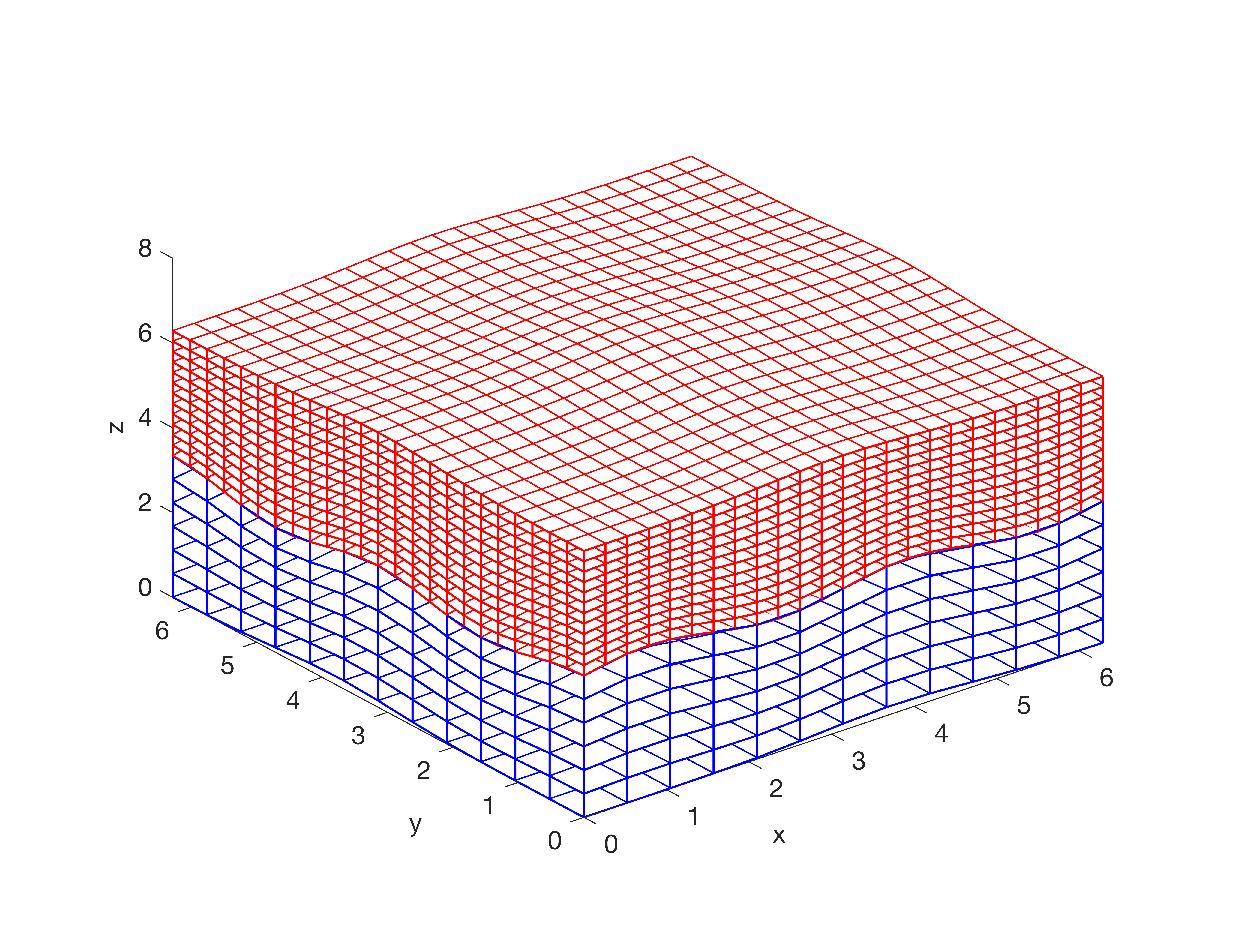
\includegraphics[width=0.6\textwidth,trim={0.4cm 0.7cm 0.8cm 1.4cm}, clip]{physical_discretization.eps}
	\caption{The sketch for the spatial discretization of physical domain $\Omega$. The blue region is the spacial discretization of coarse subdomain $\Omega^c$ and the red region is the spatial discretization of fine domain $\Omega^f$.}\label{physical_discretization}
\end{figure}

In this section, we discretize the elastic wave equation (\ref{elastic_curvi}) with mesh refinement interface $\Gamma$. Without losing generality, we assume the ratio of mesh sizes for subdomain $\Omega^f_r$ and subdomain $\Omega^c_r$ is $1:2$, that is the mesh sizes of $\Omega_r^f$ and $\Omega_r^c$ satisfy
\[h_1(n_1^h-1) = 1, \ \ \ h_2(n_2^h-1) = 1, \ \ \ h_3(n_3^h-1) = 1\]
and
\[2h_1(n_1^{2h}-1) = 1, \ \ \ 2h_2(n_2^{2h}-1) = 1, \ \ \ 2h_3(n_3^{2h}-1) = 1\]
respectively, other ratios can be treated analogously. Figure \ref{physical_discretization} gives an illustration of the discretation of a physical domain. 

We focus on the numerical treatment of the interface conditions (\ref{interface_cond}) and suppose boundaries are periodic in directions $1$ and $2$, ignore the boundaries in dierection $3$. In Figure \ref{section_discretization}, we fix $x^2 = 0$ and present the $x^1$-$x^3$ section of the domain $\Omega$ in both curvilinear space and parameter space.
\begin{figure}[htbp]
	\centering
	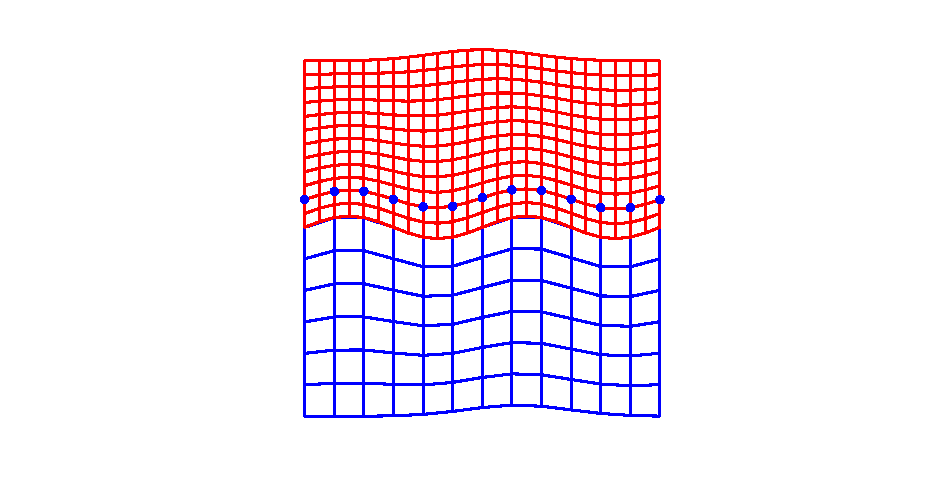
\includegraphics[width=0.45\textwidth,trim={1.0cm 2.0cm 1.0cm 1.8cm}, clip]{physical_section_discretization.eps}
	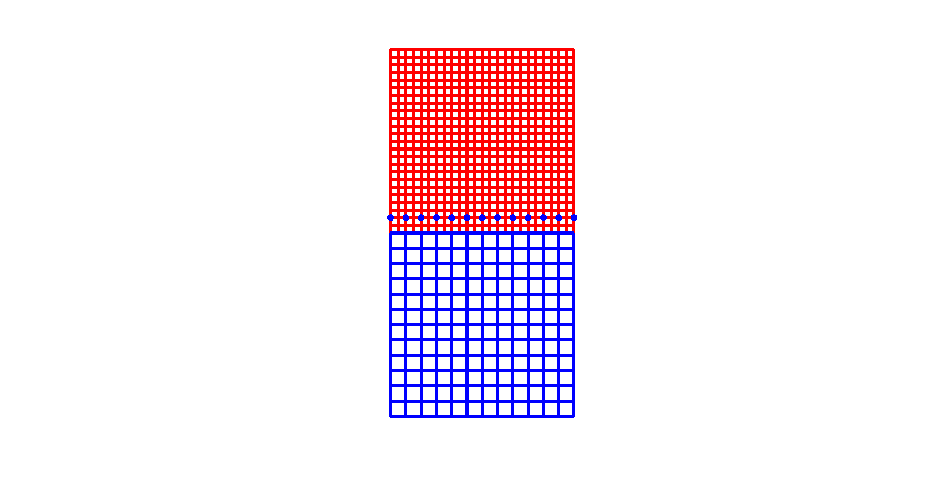
\includegraphics[width=0.45\textwidth,trim={1.0cm 2.0cm 1cm 1.8cm}, clip]{parameter_section_discretization.eps}
	\caption{The sketch of spacial discretization of $x^1$-$x^3$ section with $x^2 = 0$. From the left to the right are for physcail domain and parameter space respectively. The blue dots are the ghost points for coarse domain $\Omega^c$.}\label{section_discretization}
\end{figure}
 To condense notations, we intoduce the multi-index notations
\[{\bf i} = (i,j,k),\ \ {\bf r}_{\bf i} = (r^1_i,r^2_j,r^3_k),\ \ {\bf x}^{\{f,c\}}_{\bf i} = (x^{\{f,c\},1}_i,x^{\{f,c\},2}_j,x^{\{f,c\},3}_k),\ \ {\bf x}_{\bf i}^{\{f,c\}} = {\bf X}^{\{f,c\}}({\bf r}_{\bf i}).\]
Note that for ${\bf x}^f_{\bf i}\in\Omega^f$, we have $i\in[1,n_1^h]$, $j\in[1,n_2^h]$, $k\in[1,n_3^h]$; for ${\bf x}^c_{\bf i}\in\Omega^c$, we have $i\in[1,n_1^{2h}]$, $j\in[1,n_2^{2h}]$, $k\in[1,n_3^{2h}]$; for ${\bf x}_{\bf i}^c \in \Gamma\cap\Omega^c$, we have $i\in[1,n_1^{2h}]$, $j\in[1,n_2^{2h}]$, $k = n_3^{2h}$; for ${\bf x}_{\bf i}^f \in \Gamma\cap\Omega^f$, we have $i\in[1,n_1^h]$, $j\in[1,n_2^h]$, $k = 1$; for ${\bf x}_{\bf i}^f\in \Omega \setminus \Omega^c := \overline{\Gamma^f}$, we have $i\in[1,n_1^h]$, $j\in[1,n_2^h]$, $k\in[2,n_3^h]$. Now, denote the grid functions in $\Omega^f$ and $\Omega^c$ as
\[{\bf f} = ({\bf f}^1, {\bf f}^2, {\bf f}^3)^T\ \ \ \ \mbox{and}\ \ \ \  {\bf c} = ({\bf c}^1, {\bf c}^2, {\bf c}^3)^T\]
respectively. Here, 
\[{\bf f}^l\approx F_l({\bf r}), \ \ {\bf X}^f({\bf r})\in\Omega^f,\ \ l=1,2,3 ,\]
and
\[{\bf c}^l \approx C_l({\bf r}),\ \ {\bf X}^c({\bf r})\in\Omega^c \ \ l = 1,2,3.\]
Furthermore, we define ${\bf f}_{\Gamma}$ as the fine grid function for ${\bf X}^f({{\bf r}})\in\Gamma$, ${\bf c}_{\Gamma}$ to be the coarse grid function for ${\bf X}^c({{\bf r}})\in\Gamma$ and ${\bf f}_{\overline{\Gamma}}$ as the fine grid function for ${\bf X}^f({{\bf r}})\in\overline{\Gamma^f}$. Particularly, we define $\wt{\bf c} = (\wt{\bf c}^1,\wt{\bf c}^2,\wt{\bf c}^3)^T$ as the coarse grid function which contains both grids in $\Omega^c$ and ghost points outside of $\Omega^c$ with $i\in[1,n_1^{2h}], j\in[1,n_2^{2h}], k\in[0,n_3^{2h}+1]$. Then we approximate the elastic wave equation (\ref{elastic_curvi}) on $\Omega^c$ by
\begin{equation}\label{elastic_semi_c}
{\varrho}^{2h} {\bf c}_{tt} =( \mathcal{ J}^{2h})^{-1}\left(\sum_{l=1}^2\mathcal{G}_l^{2h}({N}_{ll}){\bf c}+\wt{\mathcal{G}}_3^{2h}({N}_{33}){\wt{\bf c}}+\sum_{l=1}^3\sum_{m=1,m\neq l}^3\mathcal{D}_l^{2h}(\mathcal{N}_{lm}^{2h}\mathcal{D}_m^{2h}{\bf c})\right) := \wt{\mathcal{L}}^{2h} {\wt {\bf c}},
\end{equation}
where 
\begin{align}\label{rho_j}
\varrho^{2h} = \left(\begin{array}{ccc}
{\bm \rho}^{2h}& ~  & ~ \\
~ & {\bm \rho}^{2h} & ~ \\
~ &~  &{\bm \rho}^{2h}\end{array}\right),\ \ \ \mathcal{J}^{2h} = \left(\begin{array}{ccc}
{\bf J}^{2h}& ~  & ~ \\
~ & {\bf J}^{2h} & ~ \\
~ &~  &{\bf J}^{2h}\end{array}\right)
\end{align}
with both ${\bm \rho}^{2h}$ and ${\bf J}^{2h}$ are $n_1^{2h}n_2^{2h}n_3^{2h}\times n_1^{2h}n_2^{2h}n_3^{2h}$ diagonal matrices with diagonal entries are values of density function $\rho^c$ and Jacobian of transformation $J^c$ on the grids in $\Omega^c$ respectively.
And $\mathcal{G}_l^{2h}({N}_{ll})$, $l=1,2$ are defined as
\begin{align}\label{g1122}
\mathcal{G}^{2h}_l({N}_{ll}) = \left(\begin{array}{ccc}
G_l^{2h}(N_{ll}^{11}) & G_l^{2h}(N_{ll}^{12})  & G_l^{2h}(N_{ll}^{13}) \\
G_l^{2h}(N_{ll}^{21}) & G_l^{2h}(N_{ll}^{22})  & G_l^{2h}(N_{ll}^{23}) \\
G_l^{2h}(N_{ll}^{31}) & G_l^{2h}(N_{ll}^{32})  & G_l^{2h}(N_{ll}^{33}) \end{array}\right),
\end{align}
with $G_l^{2h}(N_{ll}^{ij})$, $i,j = 1,2,3$, are $n_1^{2h}n_2^{2h}n_3^{2h}\times n_1^{2h}n_2^{2h}n_3^{2h}$ matrices which are from the central difference operator for second derivative with variable coefficient in direction $l$, the superscript $ij$ represents the $i'$th row and $j'$th column of matrix $N_{ll}$, and $N^{ij}_{ll}$ is a function of ${\bf r}$ located in coarse parameter domain. As for $\wt{\mathcal{G}}_3^{2h}({N}_{33})$, it has a structure
\[ \wt{\mathcal{G}}^{2h}_3({N}_{33}) = \left(\begin{array}{ccc}
\wt{G}_3^{2h}(N_{33}^{11}) & \wt{G}_3^{2h}(N_{33}^{12})  & \wt{G}_3^{2h}(N_{33}^{13}) \\
\wt{G}_3^{2h}(N_{33}^{21}) & \wt{G}_3^{2h}(N_{33}^{22})  & \wt{G}_3^{2h}(N_{33}^{23}) \\
\wt{G}_3^{2h}(N_{33}^{31}) & \wt{G}_3^{2h}(N_{33}^{32})  & \wt{G}_3^{2h}(N_{33}^{33}) \end{array}\right),\]
where $\wt{G}_3^{2h}(N_{33}^{ij})$, $i,j = 1,2,3$, are $n_1^{2h}n_2^{2h}n_3^{2h}\times n_1^{2h}n_2^{2h}(n_3^{2h}+2)$ matrices which are defined as in (\ref{sbp_2nd_1}) for direction $3$, and $N_{33}^{ij}$ is a function of ${\bf r}$ located in coarse parameter domain. Finally, let's look at the term $\mathcal{D}_l^{2h}(\mathcal{N}_{lm}^{2h}\mathcal{D}_m^{2h})$, $l = 1,2,3, m = 1,2,3, l\neq m$, we use $\mathcal{D}_1^{2h}(\mathcal{N}_{12}^{2h}\mathcal{D}_2^{2h})$ as an example and other cases are analogous,
\begin{equation}\label{D12}
\mathcal{D}_1^{2h} = {\bf I}\otimes D_1^{2h} \otimes {\bf I}_2 \otimes {\bf I}_3,\ \ \ \mathcal{D}_2^{2h} ={\bf I}\otimes {\bf I}_1\otimes D_2^{2h}\otimes {\bf I}_3,
\end{equation}
where ${\bf I}$ is a $3\times3$ identity matrix, ${\bf I}_l$, $l = 1,2,3$ are $n_l^{2h}\times n_l^{2h}$ identity matrices, $D_1^{2h}$ is a $n_1^{2h}\times n_1^{2h}$ matrix defined in (\ref{first_sbp}) for direction $1$ and $D_2^{2h}$ is a matrix of size $n_2^{2h}\times n_2^{2h}$ defined in (\ref{first_sbp}) for direction $2$. $\mathcal{N}_{12}^{2h}$ is a $3n_1^{2h}n_2^{2h}n_3^{2h}\times3n_1^{2h}n_2^{2h}n_3^{2h}$ matrix with a structure
\begin{align}\label{N12}
\mathcal{N}_{12}^{2h}= \left(\begin{array}{ccc}
\mathscr{N}_{12}^{2h,11}&\mathscr{N}_{12}^{2h,12}& \mathscr{N}_{12}^{2h,13}\\
\mathscr{N}_{12}^{2h,21} & \mathscr{N}_{12}^{2h,22} & \mathscr{N}_{12}^{2h,23} \\
\mathscr{N}_{12}^{2h,31}&\mathscr{N}_{12}^{2h,32}&  \mathscr{N}_{12}^{2h,33}\\ \end{array}\right),
\end{align}
here, $\mathscr{N}_{12}^{2h,ij}$, $i,j = 1,2,3$ are diagonal matrices of size $n_1^{2h}n_2^{2h}n_3^{2h}\times n_1^{2h}n_2^{2h}n_3^{2h}$ with the diagonal values to be $N_{12}^{ij}({\bf r})$ and ${\bf r}$ loacted in coarse parameter domain. Next, we approximate the elastic wave equation (\ref{elastic_curvi}) on $\overline{\Gamma^f}$ 
\begin{equation}\label{elastic_semi_f}
\varrho^h_{\overline{\Gamma}} ({\bf f}_{\overline{\Gamma}})_{tt} =
( \mathcal{ J}_{\overline{\Gamma}}^{h})^{-1}\left(\sum_{l=1}^3\Big(\big(\mathcal{G}_l^{h}({N}_{ll}){\bf f}\big)\Big|_{\overline{\Gamma}}+\sum_{m=1,m\neq l}^3\big(\mathcal{D}_l^{h}(\mathcal{N}_{lm}^{h}\mathcal{D}_m^{h}{\bf f})\big)\Big|_{\overline{\Gamma}}\Big)\right) := \mathcal{L}^h{\bf f}\Big|_{\overline{\Gamma}},
\end{equation}
where ${\varrho}^{h}_{\overline{\Gamma}}$ and ${\mathcal{J}}^{h}_{\overline{\Gamma}}$ are $3n_1^hn_2^h(n_3^h-1)\times 3n_1^hn_2^h(n_3^h-1)$ diagonal matrices, which have similar definitions as in (\ref{rho_j}), but correspond to the grids in $\overline{\Gamma^f}$. Lastly, we approximate the elastic wave equation (\ref{elastic_curvi}) on $\Gamma$ with fine grid points by
\begin{equation}\label{elastic_semi_f_i}
{\varrho}^h_\Gamma ({\bf f}_\Gamma)_{tt} =
( {\mathcal{ J}}^{h}_\Gamma)^{-1}\left(\sum_{l=1}^3\Big(\big(\mathcal{G}_l^{h}({N}_{ll}){\bf f}\big)\Big|_\Gamma+\sum_{m=1,m\neq l}^3\big(\mathcal{D}_l^{h}(\mathcal{N}_{lm}^{h}\mathcal{D}_m^{h}{\bf f})\big)\Big|_\Gamma\Big) \right) + {\bm \eta} := \mathcal{L}^h{\bf f}\Big|_\Gamma + {\bm \eta},
\end{equation}
with 
\begin{equation}\label{eta}
{\bm \eta} = {\varrho}^h_{\Gamma}\wt{\mathcal{P}}\left(\big(({ \varrho}^{2h})^{-1}\wt{\mathcal{L}}^{2h} \wt{{\bf c}}\big)\Big|_{\Gamma}\right) - \mathcal{L}^{h}{\bf f}\Big|_{\Gamma},
\end{equation}
here, ${\varrho}^{h}_{\Gamma}$ and ${\mathcal{ J}}^{h}_{\Gamma}$ are $3n_1^hn_2^h\times 3n_1^hn_2^h$ diagonal matrices with similar definitions as in (\ref{rho_j}) with fine grids on $\Gamma$. $\big(({\varrho}^{2h})^{-1}\wt{L}^{2h} \wt{{\bf c}}\big)\big|_{\Gamma}$ is a colume vector of size $3n_1^{2h} n_2^{2h}$ and its value corresponds to the coarse grids on $\Gamma$. In addition, the terms $\mathcal{G}_l^h({N}_{ll}), l = 1,2$ and $\mathcal{D}_l^h(\mathcal{N}_{lm}^h\mathcal{D}_m^h), l=1,2,3,m=1,2,3,l\neq m$ in (\ref{elastic_semi_f})--(\ref{elastic_semi_f_i}) have similar definitions as in (\ref{g1122})--(\ref{N12}), and $\mathcal{G}_3^h({N}_{33})$ is defined by
\[ \mathcal{G}^{h}_3({N}_{33}) = \left(\begin{array}{ccc}
G_3^{h}(N_{33}^{11}) & G_3^{h}(N_{33}^{12})  & G_3^{h}(N_{33}^{13}) \\
G_3^{h}(N_{33}^{21}) & G_3^{h}(N_{33}^{22})  & G_3^{h}(N_{33}^{23}) \\
G_3^{h}(N_{33}^{31}) & G_3^{h}(N_{33}^{32})  & G_3^{h}(N_{33}^{33}) \end{array}\right),\]
where ${G}_3^{h}(N_{33}^{ij}({\bf r}))$, $i,j = 1,2,3$, are $n_1^{h}n_2^{h}n_3^{h}\times n_1^{h}n_2^{h}n_3^{h}$ matrices which are defined as in (\ref{sbp_2nd_2}) for direction $3$, and ${\bf r}$ locates in the fine parameter space. For the simplicity of analysis, we introduce a general notation for the schemes (\ref{elastic_semi_f}) and (\ref{elastic_semi_f_i}) in the fine domain $\Omega^f$,
\begin{align}\label{fine_scheme}
{\varrho}^h{\bf f}_{tt} = \hat{\mathcal{L}}^h{\bf f} = \left\{
\begin{aligned}
&\mathcal{L}^h{\bf f}\big|_\Gamma +{\bm \eta}, \\
&\mathcal{L}^h{\bf f}\big|_{\overline{\Gamma}}.
\end{aligned}
\right.
\end{align}
In the following we are going to look at the interpolation operator ${\bf P}$ and restriction operator ${\bf R}$ in two dimensions. The stencils for the interpolation operator ${\bf P}$ can be easily computed by a Talor series expansion. In our case, we have the ratio of the mesh sizes for subdomain $\Omega^f$ and $\Omega^c$ is $1:2$, then if  ${\bf P}$ is a fourth order interpolation operator in two dimensions,  the stencils of ${\bf P}$ are illuatrated in  Figure \ref{interpolation}, the stencils for the corresponding restriction operator $\bf R$ in two dimensions can be determined by the compatibility between interpolation and restriction operators, ${\bf P} = 4{\bf R}^T$, and its stencil is presented in Figure \ref{restriction}.
\begin{figure}[htbp]
	\centering
	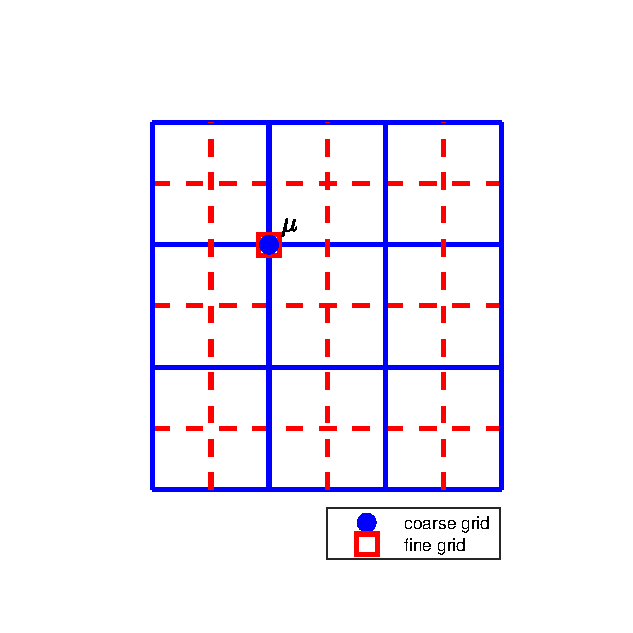
\includegraphics[width=0.24\textwidth,trim={1.8cm 0.8cm 1.4cm 1.2cm}, clip]{interpolation1.eps}
	\includegraphics[width=0.24\textwidth,trim={1.8cm 0.8cm 1.4cm 1.2cm}, clip]{interpolation2.eps}
	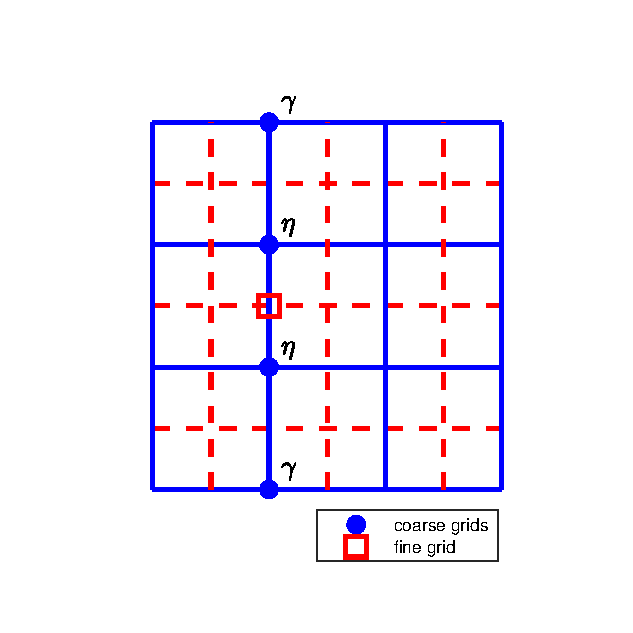
\includegraphics[width=0.24\textwidth,trim={1.8cm 0.8cm 1.4cm 1.2cm}, clip]{interpolation3.eps}
	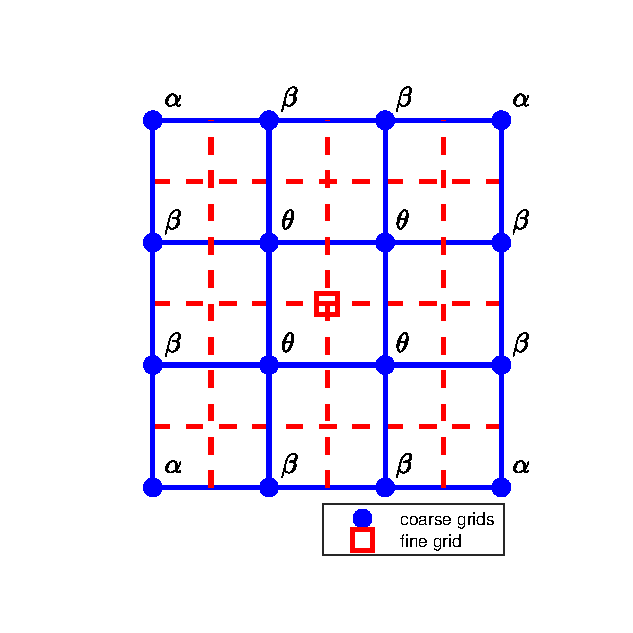
\includegraphics[width=0.24\textwidth,trim={1.8cm 0.8cm 1.4cm 1.2cm}, clip]{interpolation4.eps}
	\caption{The sketch for the stencils of fourth order interpolation operator ${\bf P}$ in two dimensions with parameters $\gamma = -\frac{1}{16}$, $\eta = \frac{9}{16}$, $\mu = 1$, $\alpha = \frac{1}{256}$, $\beta = -\frac{9}{256}$ and $\theta = \frac{81}{256}$. }\label{interpolation}
\end{figure}
\begin{figure}[htbp]
	\centering
	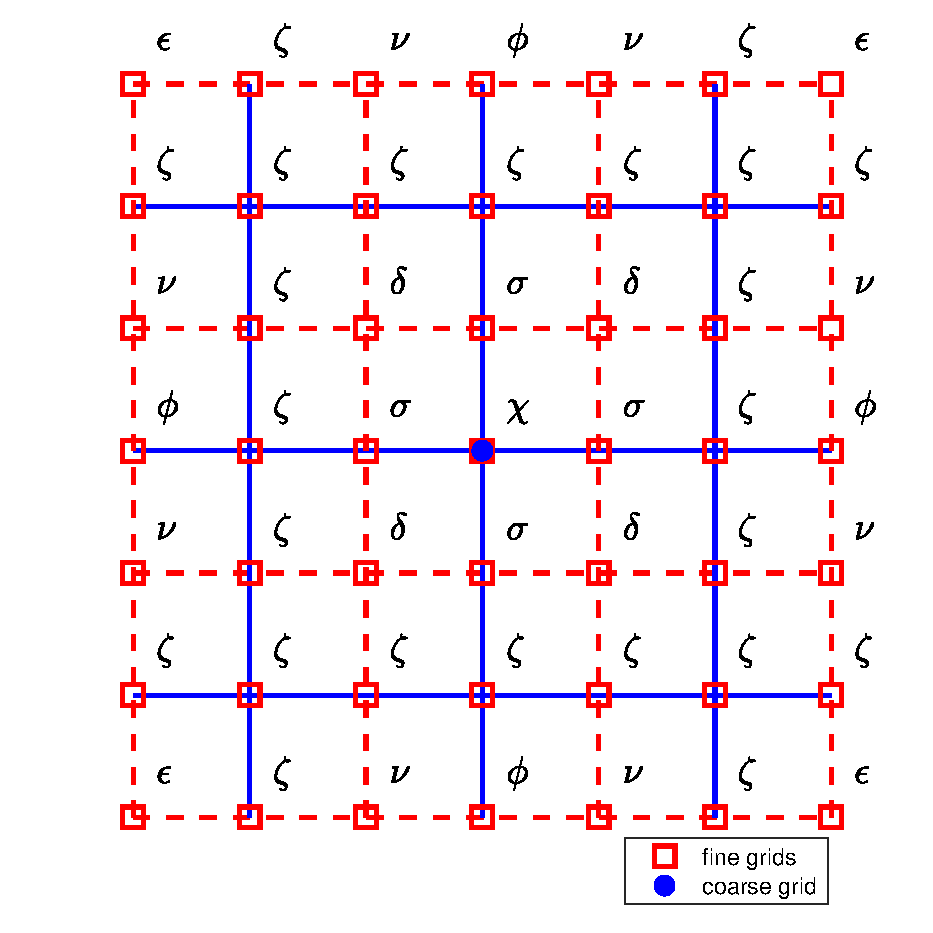
\includegraphics[width=0.6\textwidth]{restriction.eps}
	\caption{The scketch for the stencil of fourth order restriction operator ${\bf R}$ in two dimensions with parameters $\epsilon = \frac{1}{1024}$, $\nu = -\frac{9}{1024}$, $\phi = -\frac{16}{1024}$, $\delta = \frac{81}{1024}$, $\sigma = \frac{144}{1024}$, $\chi = \frac{256}{1024}$ and $\zeta = 0$.}\label{restriction}
\end{figure}

To proceed the interface conditions (\ref{interface_cond}), we fisrtly introduce scaled interpolation and restriction operators
\[\wt{\mathcal{P}} = (\mathcal{J}^h_\Gamma \mathscr{R}^h)^{-\frac{1}{2}}\mathcal{P}(\mathcal{J}^{2h}_\Gamma \mathscr{R}^{2h})^{\frac{1}{2}},\ \ \ \ \wt{\mathcal{R}} =  (\mathcal{J}^{2h}_\Gamma \mathscr{R}^{2h})^{-\frac{1}{2}}\mathcal{R}(\mathcal{J}^{h}_\Gamma \mathscr{R}^h)^{\frac{1}{2}}.\]
Here, $\mathscr{R}^{h}$ is a diagonal matrix of size $n_1^{h}n_2^h\times n_1^hn_2^h$ and its diagonal value is $|\nabla_x^f r^3|$ evalued at the fine grid points on interface $\Gamma$; similarly, $\mathscr{R}^{2h}$ is a diagonal matrix of size $n_1^{2h}n_2^{2h}\times n_1^{2h}n_2^{2h}$ and its diagonal value is $|\nabla_x^c r^3|$ evalued at the coarse grid points on interface $\Gamma$. Beisdes, $\mathcal{P}$ is a $3n_1^{2h}n_2^{2h}n_3^{2h}\times 3n_1^{2h}n_2^{2h}n_3^{2h}$ matrix and $\mathcal{R}$ is a $3n_1^hn_2^hn_3^h\times 3n_1^hn_2^hn_3^h$ matrix with the following stuctures 
\begin{align}\label{iandr}
\mathcal{P} = \left(\begin{array}{ccc}
{\bf P}& ~  & ~ \\
~ & {\bf P} & ~ \\
~ &~  &{\bf P}\end{array}\right),\ \ \ \mathcal{R} = \left(\begin{array}{ccc}
{\bf R}& ~  & ~ \\
~ & {\bf R} & ~ \\
~ &~  &{\bf R}\end{array}\right),
\end{align}
where $\bf P$ is a $n_1^{2h}n_2^{2h}n_3^{2h}\times n_1^{2h}n_2^{2h}n_3^{2h}$ matrix which has stencils as in Figure \ref{interpolation} and $\bf R$ is a $n_1^hn_2^hn_3^h\times n_1^hn_2^hn_3^h$ matrix with a stencil as in Figure \ref{restriction}. Lastly, $\mathcal{J}^{2h}_\Gamma$ has a similar definition as $\mathcal{J}^{2}_\Gamma$, but it is evaluated at the coarse grids on interface $\Gamma$.

Now, we are ready to state the continuous interface conditions (\ref{interface_cond}), the grid functions ${\bf f}$ and ${\bf c}$ are coupled through interface conditions,
\begin{equation}\label{continuous_sol}
{\bf f}_{\Gamma} = \wt{\mathcal{P}}({\bf c}_{\Gamma}),
\end{equation}
which imposes the continuity of the solution at the interface $\Gamma$
and
\begin{equation}\label{continuous_traction}
(\mathscr{R}^{2h}{\mathcal J}_{\Gamma}^{2h})^{-1}\big(\wt{\mathcal{A}}_3^{2h}\wt{\bf c}\big)\big|_\Gamma
= \wt{\mathcal{R}}\left((\mathscr{R}^{h}{\mathcal J}^h_{\Gamma})^{-1}((\mathcal{A}_3^h{\bf f})\big|_\Gamma-h_3\omega_1{\mathcal J}^h{\bm \eta})\right)
\end{equation}
where we have used the notations
\begin{equation}\label{hatAf}
(\mathcal{A}_3^h{\bf f})\big|_\Gamma = (\mathcal{N}_{31}^{h}\mathcal{D}^h_1{\bf f})\big|_\Gamma + (\mathcal{N}_{32}^h\mathcal{D}^h_2{\bf f})\big|_\Gamma + (\mathcal{N}_{33}^h\mathscr{D}_3^h{\bf f})\big|_\Gamma,
\end{equation}
and
\begin{equation}\label{hatAc}
(\wt{\mathcal{A}}_3^{2h}\wt{\bf c})\big|_\Gamma = (\mathcal{N}_{31}^{2h}\mathcal{D}^{2h}_1{\bf c})\big|_\Gamma + (\mathcal{N}_{32}^{2h}\mathcal{D}^{2h}_2{\bf c})\big|_\Gamma + (\mathcal{N}_{33}^{2h}\wt{\mathscr D}^{2h}_3\wt{\bf c})\big|_\Gamma,
\end{equation}
 which imposes the continuity of traction at the interface $\Gamma$, here, $\omega_1$ is the first entry in the scalar product (\ref{inner_product}), $\wt{\mathscr{D}}_3^{2h}$ is defined as
 \[\wt{\mathscr{D}}_3^{2h} = {\bf I}\otimes {\bf I}_1 \otimes {\bf I}_2 \otimes \wt{\mathfrak{D}}_3^{2h}\]
 where ${\bf I}$ is a $3\times3$ identity matrix, ${\bf I}_l$, $l = 1,2$ are $n_l^{2h}\times n_l^{2h}$ identity matrices, $\wt{\mathfrak{D}}_3^{2h}$ is a $n_3^{2h}\times (n_3^{2h}+2)$ matrix defined in (\ref{sbp_1st_1}) for direction $3$, and $\mathscr{D}_3^{h}$ is defined as
 \[\mathscr{D}_3^{h} = {\bf I}\otimes {\bf I}_1 \otimes {\bf I}_2 \otimes \wt{\mathfrak{D}}_3^{2h}\]
 where ${\bf I}$ is a $3\times3$ identity matrix, ${\bf I}_l$, $l = 1,2$ are $n_l^{h}\times n_l^{h}$ identity matrices, $\mathfrak{D}_3^{h}$ is a $n_3^{h}\times n_3^{h}$ matrix defined in (\ref{sbp_1st_2}) for direction $3$.
 
 Note that both (\ref{sbp_1st_1}) and (\ref{sbp_1st_2}) are defined only on boundaries, but for the dimension consistency, we define $\wt{\mathfrak{D}}^{2h}_3$ and $\mathfrak{D}^h_3$ for the whole coarse domain and fine domain respectively. As for the elements in $\wt{\mathfrak{D}}^{2h}_3$ and $\mathfrak{D}^h_3$ which do not correspond to the coarse grid points and fine points on the interface $\Gamma$, we can set they are to be zeros, since we are not using them in analysis.

